\section{Components}
Chapter \ref{cha:technologies} examined the various components viable for use in the nodes. This section contains the decisions made regarding the components.

Both Arduino Uno and Mega are used in the solution, as they qualify regarding specifications, and due to their availability to the project group. The Mega boards are not faster, but can contain more program code and allow for more components. Although not necessary, but the devices are used as they are available.

The Raspberry Pi B+ model is used in the solution as the main node and handler of data, based on the need to store, handle, and present data.  This device has the capability to display and power user interfaces and show the data received from the sensors, as it has more processing power than the Arduinos, and the ports needed to add a screen. The B+ model is used as it is available to the project group.

The data that is chosen to monitor with sensors in the solution is the moisture of the ground. This has been chosen, as the two alternatives, pH and compaction, are changing at a slower pace, and is more expensive in regards to sensors.

The communication device chosen for this project is the nRF24L01, as it is sufficient, and because of its documentation, price, and low power usage. The shorter range is not a problem, as the nodes is used in a relay network. The transfer speed of the module is also good enough for the requirements, which makes this module good for the solution described in the report.

With the components chosen and the datasheets examined, the nodes will be connected as seen on Figure \ref{fig:compsketch}.

\begin{figure}[!h]
	\centering
	\makebox[\textwidth][c]{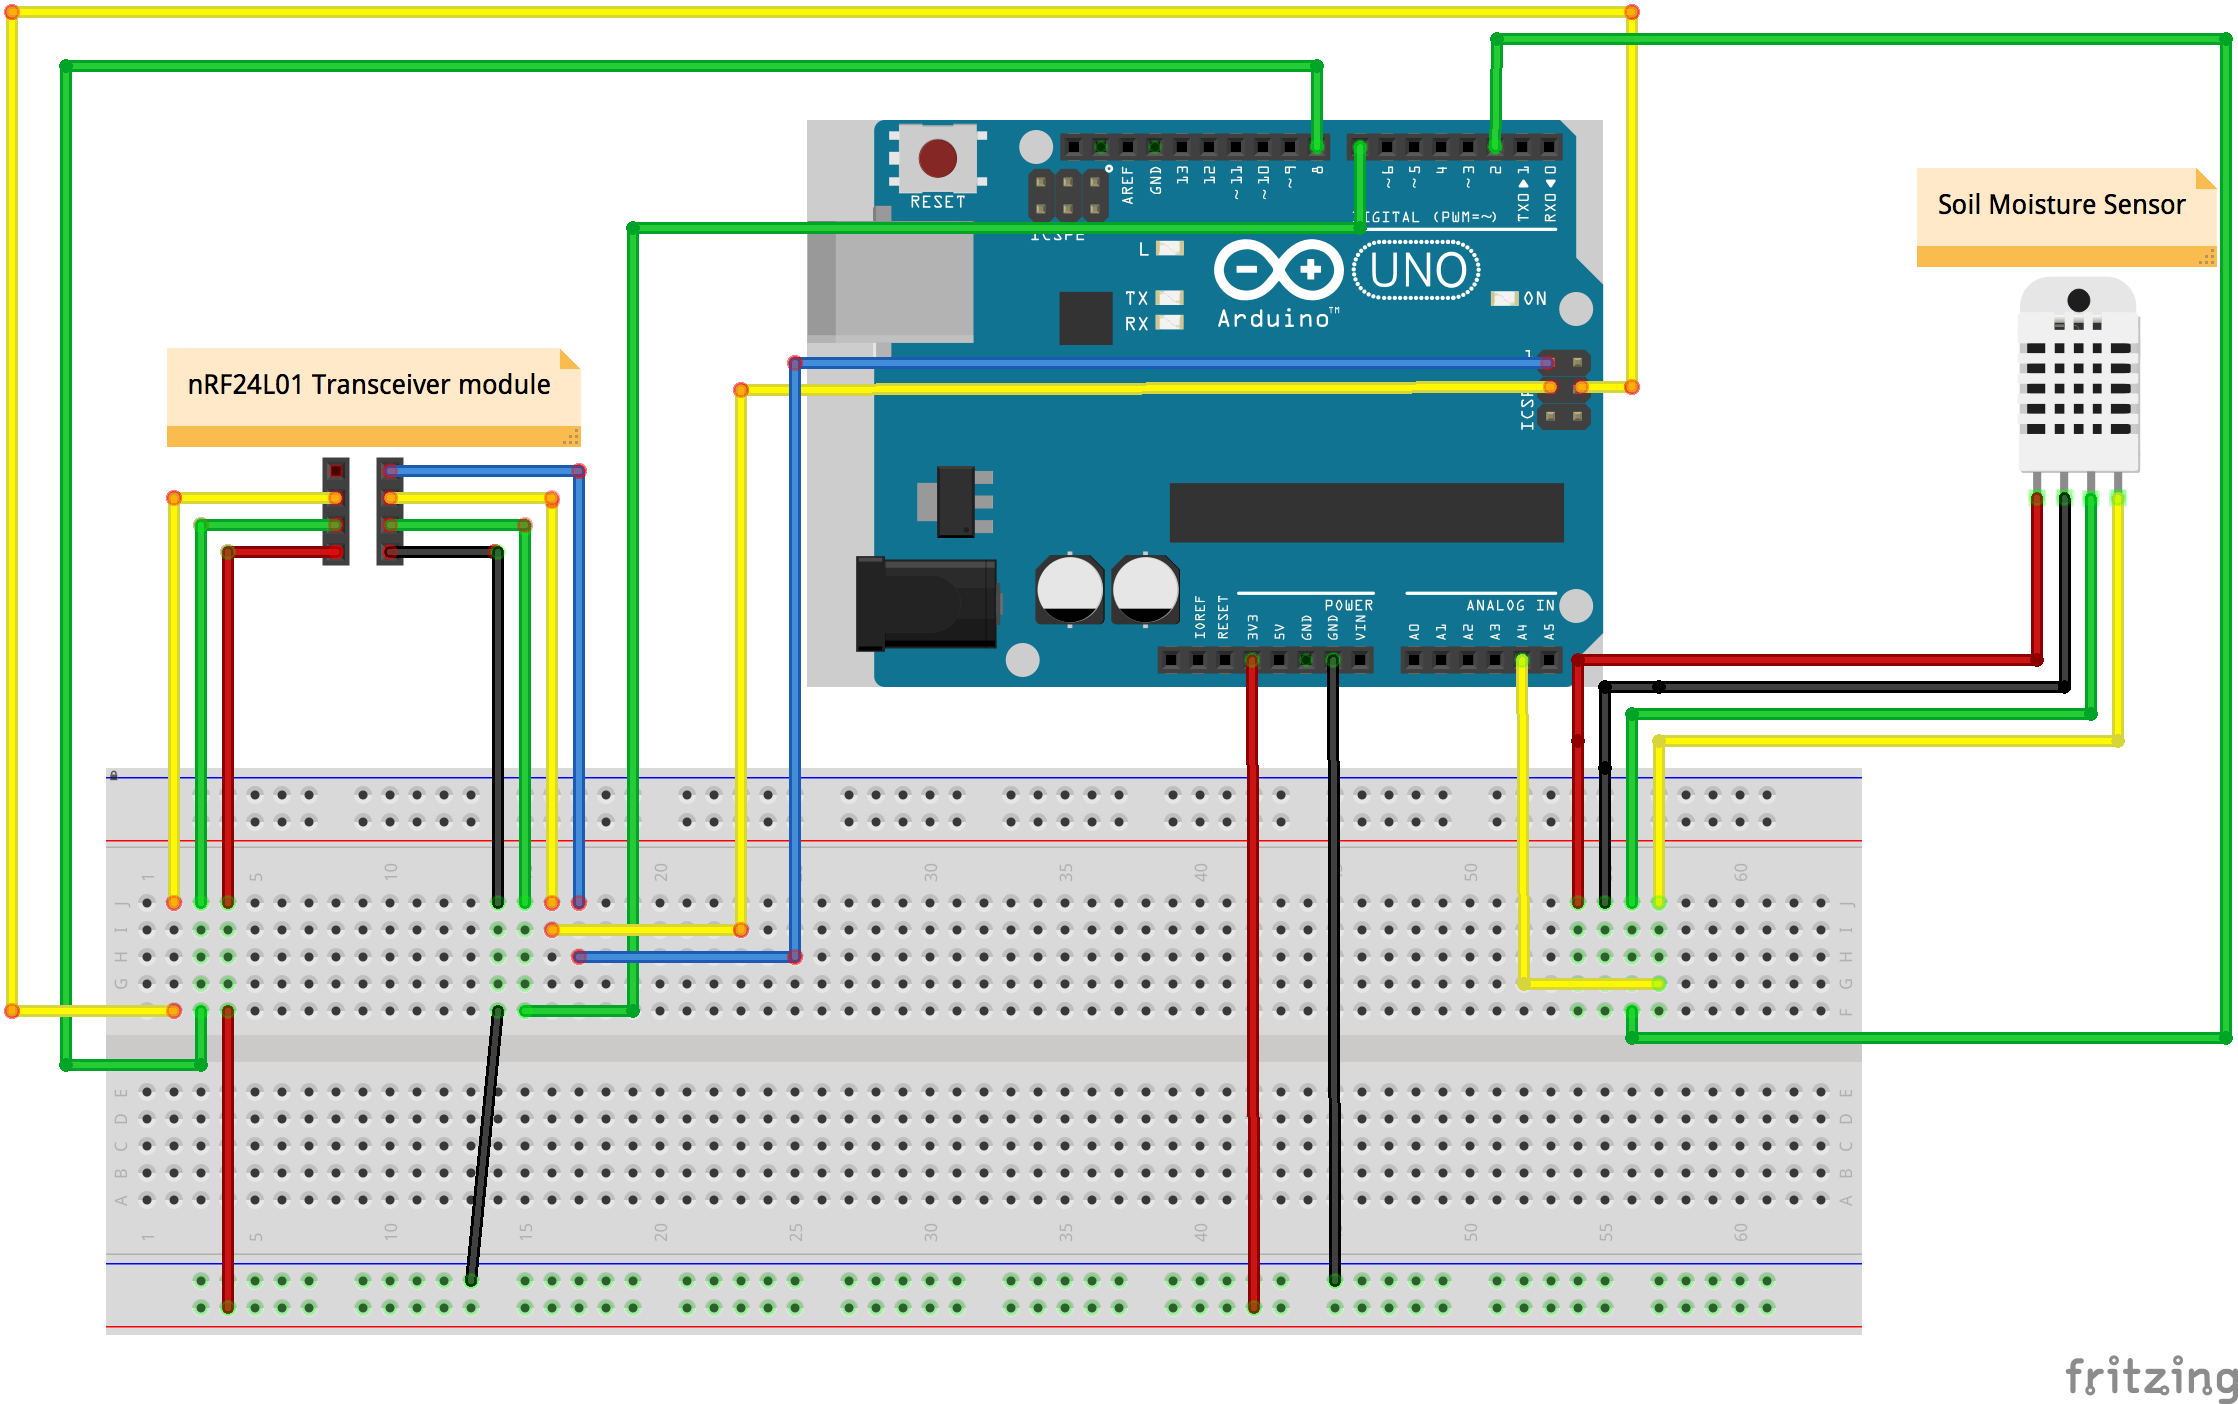
\includegraphics[width=1\textwidth]{chapters/design/figures/Sketch_bb.png}}
	\caption{Arduino connected to sensor and radio module.}
	\label{fig:compsketch}
\end{figure}

\subsection{NRF24L01 Transceiver}
The chosen radio transceiver module contains multiple features to make up for packets loss. These includes checking hashes and sending acknowledgements\cite{nf24datasheet}.
These features makes it harder to replace the radio modules in the nodes, as they are platform specific to the NRF24L01. The analysis examined the possibility of using different radio modules in case some requirements changes, which is not possible if using platform specific features. These features also causes more battery to be used, which is a problem in devices being buried, as discussed in Chapter \ref{cha:batcons}.

Because of this, these features have been disabled. This means that the radio packets does not contain a hash, nor does it send acknowledgements when packets arrives. The speed and power have also been turned down, so the device will transfer slower, and use less battery power.
